\section{Современные подходы к генерации ансамблей}

\subsection{Области применения случайных ансамблей}


Характерной чертой современного этапа развития прикладной науки является интенсивное применение компьютерных технологий в самых разных видах научных исследований. Ярким примером является теория фильтрации, изучающая закономерности движения жидкостей и газов в проницаемых структурах, некоторые из направлений исследования твёрдых тел а также электродинамики и многих других.

Жёсткие диски и сферы долгое время пользовались популярностью среди физиков, материалловедов и химиков для описания структурных. и кинетических свойств вещества. 

К середине XX в. теория фильтрации считалась сложившейся областью прикладной гидродинамики. Но оставалась неясной природа многочисленных феноменологических законов сопротивления, которые могли иметь ярко выраженный нелинейный характер. В общих чертах было ясно, что ответ на этот вопрос лежит в области микромеханики течения жидкости в пористой среде. 

Внимательное изучение подходов привело к необходимости классификации всего многообразия структурных моделей пористой среды. В основу классификации был положен известный принцип объединения различных моделей в группы на основе иерархически организованной системы признаков, характеризующих значимые особенности пористой среды. В случае стохастических структур появление хаотических режимов в фазовом пространстве такой системы практически неизбежно. Необходимость универсального подхода для описания сложнейшей структуры хаотических аттракторов потребовала подробного анализа таких понятий, как самоподобие и размерность фрактальных объектов. Перколяционные модели распространения жидкости в пористых структурах позволяют с помощью простейших закономерностей смоделировать задачу о микроструктуре неустановившегося режима фильтрационного течения, чрезвычайно сложную в рассмотрении с помощью традиционных методов моделирования.

Теория перколяции (протекания) возникла первоначально в физике твердого тела, но в последние годы находит все более широкие применения в самых различных естественных науках (физика, механика, геофизика, астрофизика, химия полимеров, коллоидная химия и т.п.). Основной объект этой теории — случайные однородные множества на графах, решетках, группах, евклидовых пространствах. При этом, в отличие от локальной теории, перколяция изучает глобальные свойства таких множеств. Именно такой подход позволяет рассмотреть широкий класс своеобразных (геометрических) фазовых переходов а также объяснить значительный спектр других физических процессов дискредитировав результат физического явления на элементы, благодаря которым данное явление произошло.

Некоторые наиболее принципиальные физические модели, приводящие к перколяционньш задачам \cite{menshikov}:

\begin{enumerate}
    \item \label{matt}
    \textbf{Фазовый переход Мотта в легированных полупроводниках.} \newline
        При легировании полупроводникового кристалла (кремния или германия), атомы которого имеют валентность 4, пятивалентными атомами (мышьяка), при достаточно высокой концентрации $\lambda>\lambda_{cr}$ пятивалентных, возникает металлическая проводимость. Качественная модель этого явления состоит в следующем. Основное состояние каждого примесного электрона в кристалле изображается некоторой поверхностью (поверхность Ферми) - Эти поверхности $S_{i}$ одинаковы, одинаково ориентированы и жестко связаны со случайно расположенными примесными атомами, локализованными в точках $x_{i}$. Их множество 1\_-|->< естественно распадается на связные компоненты $K_{j}$- Металлизация кристалла при легировании. примесью отождествляется с появлением (с вероятностью 1) бесконечного связного кластера, то есть перколяцией (протеканием).
    \item \label{distruction}
    \textbf{Концентрационная модель разрушения Журкова.} \newline
        Современная концепция разрушения однородных материалов основана на следующих представлениях. При действии на образец одноосной нагрузки в его толще возникают микротрещины (микросколы), которые можно представить в виде плоских дисков. «Близко расположенные» трещины объединяются, происходит их укрупнение. Простейший критерий укрупнения (не учитывающий взаимную ориентацию микротрещин) состоит в следующем. Окружим каждую трещину сферой $S_{i}$, диаметр которой в $3$ раза превосходит диаметр соответствующего диска и имеющей тот же самый центр $x_{i}$. Если сферы, связанные с двумя микротрещинами, пересекаются, то последние сливаются. Образование магистральной трещины (то есть разрушение образца) эквивалентно тем самым появлению связного (практически бесконечного) кластера сфер, то есть перколяции «дефектного» множества.
    \item \label{aging}
    \textbf{Старение полимерных покрытий.} \newline
        В процессе эксплуатации изоляционных полимерных покрытий (кабели, провода и так далее) в них развивается сеть микродефектов или пор, появление которых может быть связано либо со структурными перестройками полимера, либо с термодиффузией низкомолекулярной компоненты (наполнителя полимерной матрицы). Для многих типов полимеров (ПВХ, эмали и так далее) элементарные микропоры имеют сферическую форму $S_{i}$. Подобно \ref{matt}, \ref{distruction}, в этом случае дефектное множество описывается пуассоновской моделью сфер случайного радиуса. Важная особенность задач \ref{aging} состоит в в том, что здесь нас интересует не только вопрос о возникновении перколяции дефектного множества. в бесконечном пространстве, но и проблема больших уклонений, которые обусловливают протекание через конечный слой вещества еще до достижения перколяционного порога (по концентрации $S$).
    \item \label{averaging}
    \textbf{Теория осреднения и перколяция.} \newline
        Во многих задачах теории осреднения случайных сред также возникают перколяционные мотивы. Близкие проблемы возникают при изучении случайных сетей сопротивлений. Представим квадратную сетку $N \times N$ состоящую из $N^2$ случайных сопротивлений $\xi_{i}$ (для простоты одинаково распределенных и независимых). Если верхний и нижний ряды шунтированы, то при прохождении тока между шунтами сетка будет иметь некоторое случайное сопротивление $\rho_{N}$. Нетрудно показать, что $\rho_{N}\xrightarrow[N\rightarrow\infty]{}\rho_{eff}$ (п. н.). Предельную величину $\rho_{eff}$ можно рассматривать как эффективное среднее сопротивление одного звена сетки. Определение $\rho_{eff}$ можно рассматривать как задачу осреднения некоторой системы разностных уравнений со случайными коэффициентами (представляющей попросту запись законов Кирхгофа для узлов и элементарных ячеек сетки),
    \item \label{nanocomposites}
    \textbf{Проводимость нанокомпозитных материаллов.}
        В нанкомпозитном материале электропроводимость является функцией процентного содержания металлической проводящей фазы к непроводящей. В случае гомогенной однородной среды, плотность вектора электрического тока связана с напряжённостью коэффициентом электропроводимости, однако при переходе к гетерогенной системе, данный коэффициент принимает вид непрерывной функции радиус-вектора от некоторого начала координат. Когда неоднородности системы становятся дискретными (мультифазная система), как параметром системы следует рассматривать параметр эффективной электропроводимости, который зависит от расположения, и размеров неоднородностей. Эмпирически обнаружена нестандартная зависимость электропроводимости системы от процентного содержания металлической фазы в модели, разработанной на основании теории перколяции. На кривой эффективной электропроводимости системы присутствуют отклонения от стандартного графика перколяционной функции в сторону меньших значений. Существует гипотеза, что это вызвано влиянием оксидных оболочках вокруг частиц металла.
\end{enumerate}

Весь перечисленный спектр задач подразумевает решение задач, связанных с рассмотрением ансамблей различных форм. В случае с концентрированной моделью разрушения Журкова (пример \ref{distruction}) мы рассматриваем трещины как некоторый ансамбль из дискообразных микротрещин, соединяющихся по некоторому, поддающемуся расчёту закону. Рассматривая такой ансамбль, мы можем предсказать где потенциально появится разлом образца. Для фазового перехода Мотта в легированных полупроводниках (пример \ref{matt}) каждому элементу присваивается некоторая сферическая область, а все элементы в совокупности могут рассматриваться как ансамбль сферических объектов с некоторым заданным на этом множестве поведением. Для задачи проводимости нанокомпозитных материаллов (пример \ref{nanocomposites}) задача поиска проводящего кластера среди всех ансамблей является основной. 

Список задач, где при некоторых приближениях мы можем перейти к рассмотрению объектов как ансамблей частиц с заданным поведением огромен, в данной главе приведено только несколько примеров.  

Текст раздела.

................................................

\begin{equation}
 \begin{aligned}
  \mathbf E^h=\pm i\mathbf H^e,\quad\mathbf H^h=\mp i\mathbf E^e. % Пример жирного шрифта
 \end{aligned}
\end{equation}

.................................................

\begin{equation}            % Пример большой формулы, где нужно переносить часть выражения на другую строчку
 \label{Eeexplicit}         % Когда нужны большие скобки, их можно открывать и закрывать с помощью \left( и \right(
 \begin{aligned}            % для случая круглых скобок. Когда надо открыть скобку на одной строке, а закрыть на другой,
  \mathbf E^e=\frac{E_0e^{-i\varphi}}{(1+2i\chi)^2}\exp\left(-\frac{\xi^2}      % надо в конце первой сроки поставить \right.,
  {1+2i\chi}\right)\left\{\left(1-\frac{\xi^2}{1+2i\chi}\right)\mathbf          % а в начале следующей - \left.
  e_x+\right.\\
  \left.+\frac{\xi^2}{1+2i\chi}(\cos2\phi\,\mathbf e_x+\sin2\phi\,\mathbf e_y)\right\}
 \end{aligned}
\end{equation}
\begin{equation}
 \label{Heexplicit}
 \begin{aligned}
  \mathbf H^e=\frac{E_0e^{-i\varphi}}{(1+2i\chi)^2}\exp\left(-\frac{\xi^2}
  {1+2i\chi}\right)\left\{\left[1-\frac{\xi^2}{1+2i\chi}-\right.\right.\\
  \left.-\frac{2\Delta^2}{1+2i\chi}\left(2-\frac{4\xi^2}
  {1+2i\chi}+\frac{\xi^4}{(1+2i\chi)^2}\right)\right]\mathbf e_y-\\
  -\frac{\xi^2}{1+2i\chi}\left[1-\frac{2\Delta^2}{1+2i\chi}\left(3-\frac{\xi^2}{1+2i\chi}\right)\right]
  (\sin2\phi\,\mathbf e_x-\cos2\phi\,\mathbf e_y)-\\
  \left.-\frac{4i\Delta\xi}{1+2i\chi}
  \left(2-\frac{\xi^2}{1+2i\chi}\right)\sin\phi\,\mathbf e_z\right\}
 \end{aligned}
\end{equation}

\begin{figure}[pH]                          % Пример рисунка, состоящего из 6 картинок
\begin{minipage}[h]{0.47\linewidth}         % Создаём "маленькие" рисунки шириной 47% от ширины страницы
\center{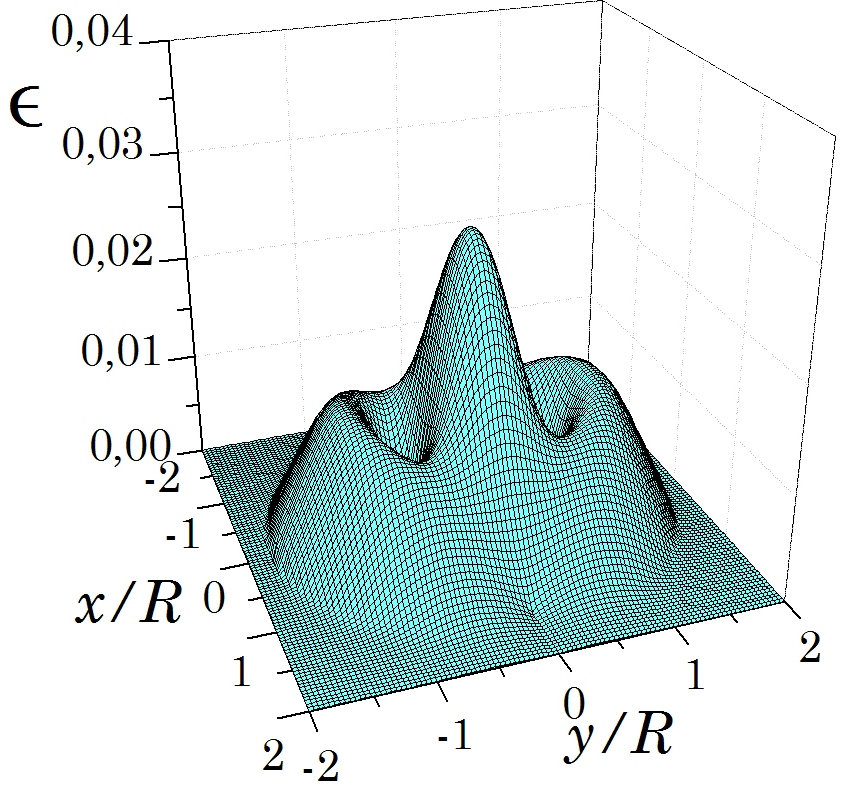
\includegraphics[width=1.0\linewidth]{images/EGraph1}} % Вставляем рисунок в полученное "окно" полностью - 100%
\end{minipage}
\hfill                                      % Следующий рисунок правее
\begin{minipage}[h]{0.47\linewidth}
\center{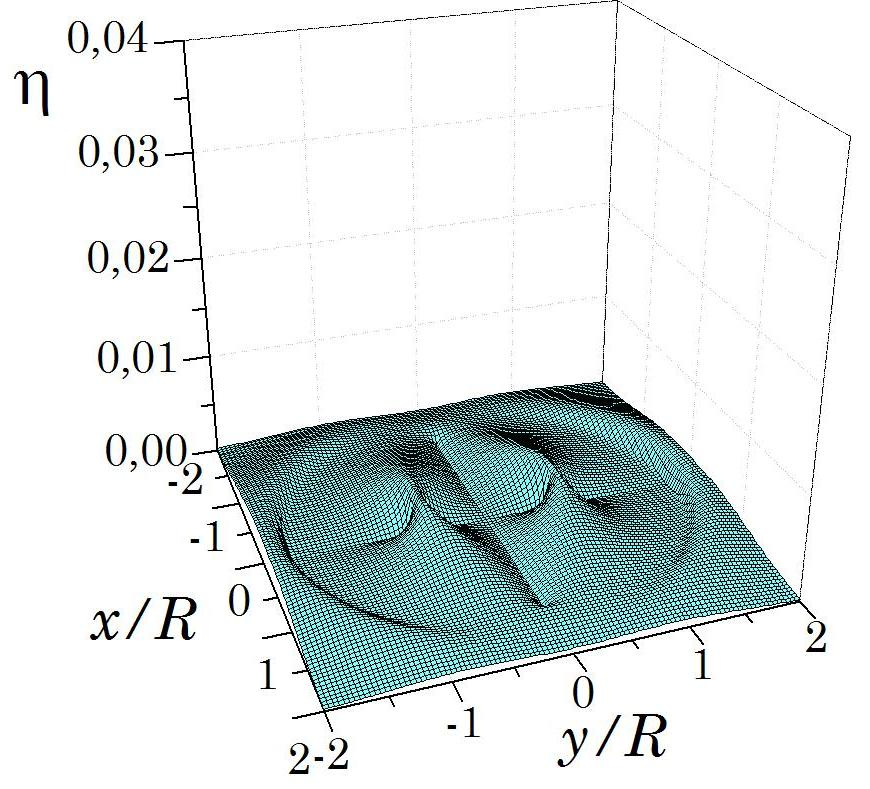
\includegraphics[width=1.0\linewidth]{images/HGraph1}}
\end{minipage}
\vfill                                      % следующий рисунок ниже - слева
\begin{minipage}[h]{0.47\linewidth}
\center{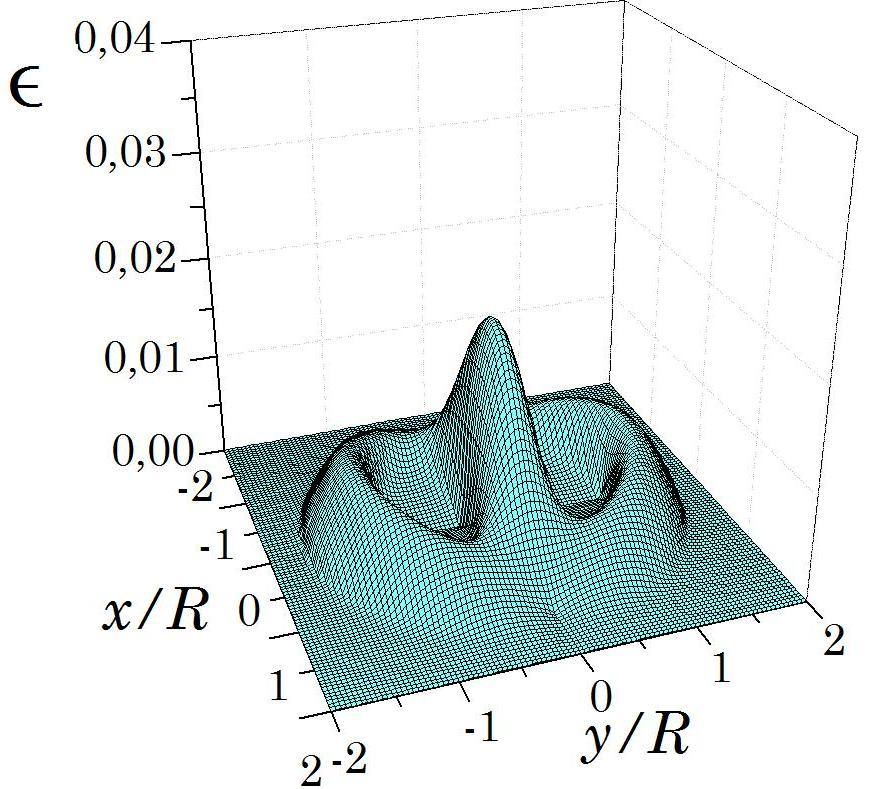
\includegraphics[width=1.0\linewidth]{images/EGraph2}}
\end{minipage}
\hfill
\begin{minipage}[h]{0.47\linewidth}
\center{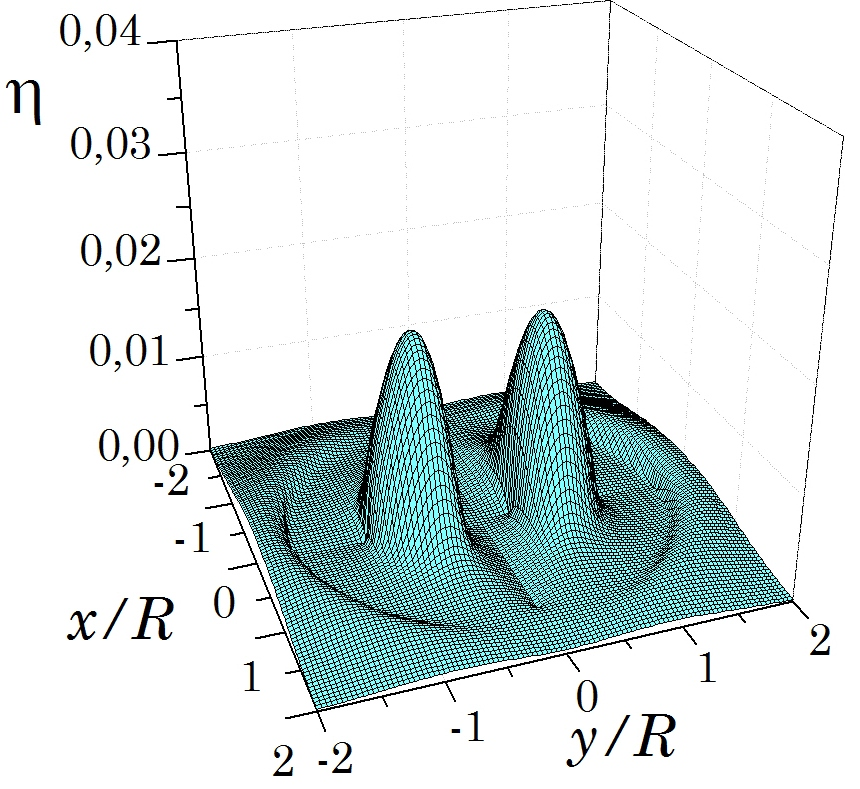
\includegraphics[width=1.0\linewidth]{images/HGraph2}}
\end{minipage}
\vfill
\begin{minipage}[h]{0.47\linewidth}
\center{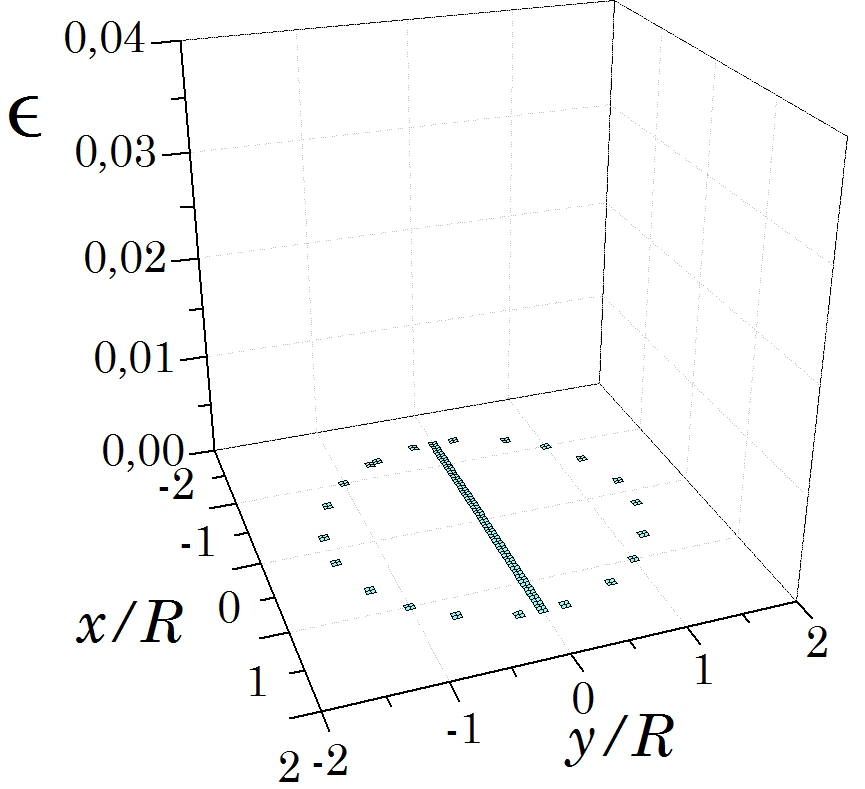
\includegraphics[width=1.0\linewidth]{images/EGraph3}}
\end{minipage}
\hfill
\begin{minipage}[h]{0.47\linewidth}
\center{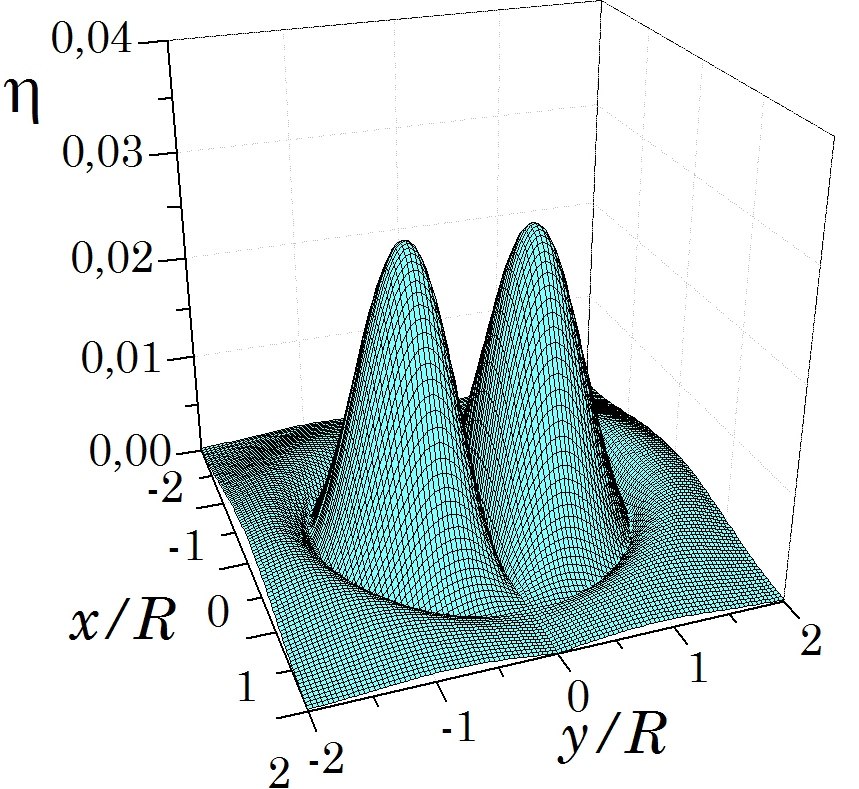
\includegraphics[width=1.0\linewidth]{images/HGraph3}}
\end{minipage}
\caption{\footnotesize Инварианты $\epsilon$ и $\eta$ для случая
одиночного линейно-поляризованного импульса $e$-типа в моменты
времени $t=0$, $t=\pi/4\omega$, $t=\pi/2\omega$. Остальные параметры
положены равными $E_0=0.1$, $z=0$, $\Delta=0.1$.} \label{EHinvs}   % Лейбл для ссылки на рисунок с помощью "рис.~\ref{EHinvs}"
\end{figure}

На рис.~\ref{EHinvs} показаны зависимости инвариантов $\epsilon$ и
$\eta$ от пространственных координат $x$ и $y$ в плоскости $z=0$ в
моменты времени $t=0$, $t=\pi/4\omega$, $t=\pi/2\omega$.
